\documentclass[UTF8,a4paper,11pt]{ctexart}

\usepackage[margin=2.35cm]{geometry}
\usepackage{graphicx}
\usepackage{booktabs}
\usepackage{enumitem}
\usepackage{fancyhdr}
\usepackage{hyperref}
\usepackage{float}

\hypersetup{colorlinks=true,linkcolor=black,urlcolor=blue}
\setlist[enumerate]{leftmargin=2.5em,itemsep=.35em,topsep=.3em}
\pagestyle{fancy}
\fancyhf{}
\fancyhead[L]{ICS Lab 1：Data Lab}
\fancyhead[R]{实验报告}
\fancyfoot[C]{\thepage}
\setlength{\headheight}{14pt}

\title{\bfseries ICS Lab 1：Data Lab 实验报告}
\author{姓名：\underline{\hspace{4cm}}\qquad 学号：\underline{\hspace{4cm}}}
\date{\today}

\begin{document}
\maketitle

\section{实验目标与环境}
本实验在 32 位补码整数模型及 IEEE 754 单精度浮点编码上完成 19 个函数。整数题需要遵守逐题给定的运算符与操作数上限；浮点题只能使用整数类型和整数运算。实现文件为 \texttt{bits.c}，使用课程提供的 \texttt{check\_ops.py} 检查规则，使用 \texttt{btest} 检查结果。

实验环境为 Ubuntu 24.04（WSL2，x86-64）。在仓库目录运行 \texttt{make clean \&\& make all}，采用 Makefile 的 \texttt{-m32 -fwrapv} 编译选项。由于当前工作副本中检查脚本的换行格式，规则检查以 \texttt{python3 check\_ops.py bits.c} 调用。

\section{实现思路}
\subsection{整数位操作与移位（P1--P9）}
\begin{enumerate}[label=\textbf{P\arabic*.}]
  \item \texttt{signMask}：将最低位的 1 左移 31 位，得到仅最高位为 1 的掩码。
  \item \texttt{bitXor}：将异或写成“仅 \(x\) 为 1”与“仅 \(y\) 为 1”两种情况的并；再利用德摩根律，把表达式改写为只含 \texttt{\textasciitilde} 与 \texttt{\&}。
  \item \texttt{negativePart}：算术右移取得符号掩码。输入为负时掩码全为 1，保留补码取负 \texttt{\textasciitilde x+1} 的结果；其余情况掩码为 0。
  \item \texttt{copyByteWithin}：将源字节右移到低 8 位并截取，用目标字节掩码清除原值，再把源字节移入目标位置。
  \item \texttt{logicalShift}：先作算术右移，再构造掩码清除符号扩展产生的高位 1。掩码写法覆盖 \(n=0\) 和 \(n=31\)，没有移位 32 位的情况。
  \item \texttt{swapNibblePairs}：构造逐字节重复的低半字节掩码 \texttt{0x0f0f0f0f}。低半字节左移 4 位，高半字节右移 4 位后合并。
  \item \texttt{secondLowestZeroBit}：令 \texttt{zeros=\textasciitilde x}，用 \texttt{zeros\&(\textasciitilde zeros+1)} 取出第一个零位对应的最低置位；消去这一位，再对余下位重复该操作。
  \item \texttt{oddParity}：依次与右移 16、8、4、2、1 位的值异或，把全部 32 位的奇偶性折叠到最低位。题目要求偶数个 1 返回 1，因此翻转该位。
  \item \texttt{rotateRightBits}：先令位数对 32 取模，分别得到无符号意义下的右移部分和左移回绕部分，再按位或合并。
\end{enumerate}

\subsection{舍入、比较与溢出（P10--P14）}
\begin{enumerate}[label=\textbf{P\arabic*.},start=10]
  \item \texttt{roundEvenPow2}：把非负输入拆成商 \(q=x\gg n\) 和余数 \(r\)。余数大于半程时商加 1；等于半程时仅在 \(q\) 为奇数时加 1，最后左移 \(n\) 位。
  \item \texttt{midpointTowardFirst}：用 \((x\mathbin{\&}y)+((x\mathbin{\oplus}y)\gg1)\) 求不溢出的向下取整中点。当中点处于两个整数之间且 \(x>y\) 时再加 1；比较时先区分符号，避免减法溢出误判。
  \item \texttt{isBetweenEitherOrder}：分别计算 \(x<a\) 与 \(x<b\)，通过操作数符号判断减法是否可能溢出。两次比较结果不同，或 \(x\) 等于任一端点，即在闭区间内。
  \item \texttt{mul5Sat}：以左移和加法计算 \(4x+x\)。先检查左移后右移能否恢复 \(x\)，再检查 \(4x+x\) 的同号加法溢出；若溢出，按输入符号选取 \texttt{INT\_MAX} 或 \texttt{INT\_MIN}。
  \item \texttt{classifyAdd3}：分两次做 32 位加法，并求每次加法的进位。将进位与三个输入的符号扩展相加，得到精确和在低 32 位之外的高位部分；再与低位和的符号比较，判断是上溢、下溢还是在范围内。
\end{enumerate}

\subsection{浮点编码与并行位操作（P15--P19）}
\begin{enumerate}[label=\textbf{P\arabic*.},start=15]
  \item \texttt{floatScaleThreeHalves}：拆出符号、阶码和尾数；对有效数字乘 3，再按所需位数右移，相当于乘 \(3/2\) 并规格化。被舍弃位按最近偶数规则进位，处理非规格化数跨入规格化区间及阶码溢出。NaN 和无穷大原样返回。
  \item \texttt{floatRoundEven}：按阶码分段。绝对值小于 \(1/2\) 时返回带原符号的零；处于 \([1/2,1)\) 时单独处理 \(1/2\) 的平局；已有整数值时原样返回。其余情况清除小数位，再根据余数与半程、整数部分奇偶性决定是否进位。
  \item \texttt{float\_i2f}：提取符号和无符号绝对值，找到最高置位以确定阶码。整数有效位不超过 24 位时直接对齐；否则截断低位并按最近偶数规则舍入，必要时处理舍入引起的阶码进位。
  \item \texttt{bitCount}：用 \texttt{0x55}、\texttt{0x33}、\texttt{0x0f} 扩展得到分组掩码；依次汇总每 2、4、8 位中的置位个数，再汇总各字节、半字，得到 32 位总数。
  \item \texttt{bitReverse}：依次交换相邻 1、2、4、8、16 位宽的分组。掩码从 \texttt{0x00ff00ff} 逐级推导，满足本题 34 次操作的上限。
\end{enumerate}

\section{检查与测试结果}
规则检查显示 19 个函数全部通过运算符及操作数检查，见图~\ref{fig:ops}。完整 \texttt{btest} 中每题 \texttt{Errors} 均为 0，总分为 \texttt{110/110}，见图~\ref{fig:btest}。这说明当前版本通过了课程提供的本地规则检查与测试。

\begin{figure}[H]
  \centering
  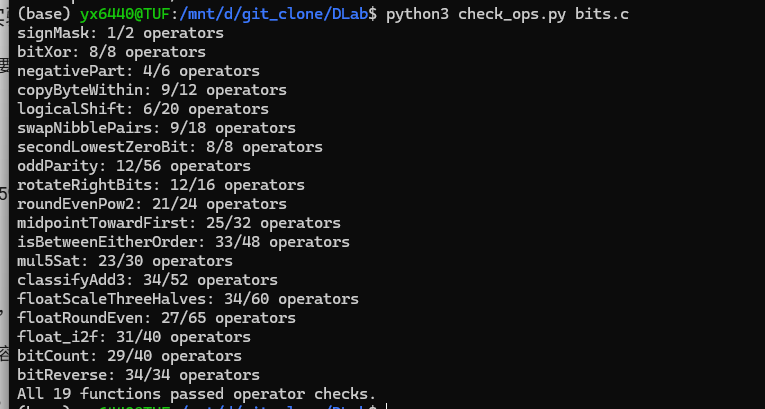
\includegraphics[width=\linewidth]{photo/.check_ops.py bits.c.png}
  \caption{\texttt{python3 check\_ops.py bits.c} 的检查结果}
  \label{fig:ops}
\end{figure}

\begin{figure}[H]
  \centering
  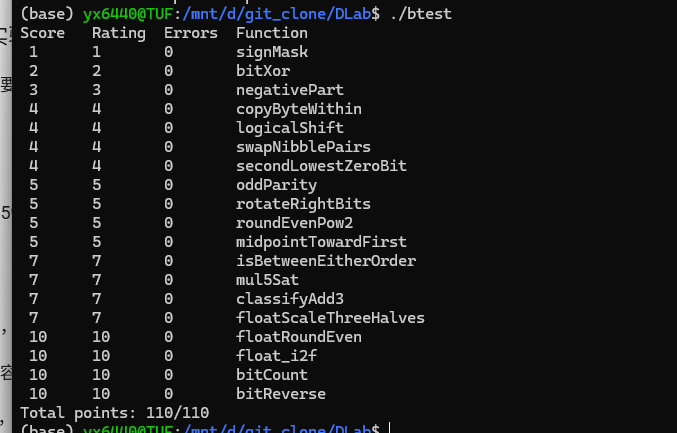
\includegraphics[width=.83\linewidth]{photo/.btest.png}
  \caption{\texttt{./btest} 的完整测试结果}
  \label{fig:btest}
\end{figure}

\section{参考资料与工具}
\begin{enumerate}
  \item 课程实验网页：\url{https://ics-26fall-fdu.github.io/labs/lab1-data-lab/}。
  \item 课程仓库中的 \texttt{README.md}、\texttt{bits.c} 题目说明及检查程序。
  \item OpenAI Codex：辅助分析题目、实现代码并整理本报告；结果使用课程检查程序核验。
\end{enumerate}

\end{document}
